\ifdefined\ishandout
\documentclass[handout]{beamer}
\else
\documentclass{beamer}
\fi

\usepackage[frenchb]{babel}
\usepackage[T1]{fontenc}
\usepackage[latin1]{inputenc}
\usepackage{hyperref}
\usepackage{multirow}
\usepackage{listings}
\usepackage{fancyvrb}
\usepackage{tikz}
\usepackage{framed}
\usepackage{algorithm}
\usepackage{algorithmic}
\usepackage{xcolor}
\usepackage{color, colortbl}
\usepackage{handoutWithNotes}

\usetikzlibrary{shapes.geometric}
\usetikzlibrary{positioning}
\usetikzlibrary{shapes.arrows, chains}
\usetikzlibrary{arrows,calc}
\usetikzlibrary{shapes.multipart}
\usepackage{array}
\usetheme{Boadilla}

\ifdefined\ishandout
\pgfpagesuselayout{3 on 1 with notes}[a4paper,border shrink=5mm]
\usecolortheme{dove}
\else
\usecolortheme{dolphin}
\fi


\lstnewenvironment{codeC}
{ \lstset{language=C,
    otherkeywords={printf,scanf}}
}
{}

\ifdefined\ishandout
\definecolor{mygreen}{rgb}{0,0,0}
\definecolor{mymauve}{rgb}{0,0,0}
\definecolor{myblue}{rgb}{0,0,0}
\else
\definecolor{mygreen}{rgb}{0,0.6,0}
\definecolor{mymauve}{rgb}{0.58,0,0.82}
\definecolor{myblue}{rgb}{0,0,1}

\fi

\definecolor{mygray}{rgb}{0.5,0.5,0.5}


\lstset{language=C,
% breakatwhitespace=false,         % sets if automatic breaks should only happen at whitespace
%  breaklines=true,                 % sets automatic line breaking
%  captionpos=b,                
commentstyle=\itshape\color{mymauve},
keywordstyle=\bfseries\color{myblue},
%numbers=left,                    % where to put the line-numbers; possible values are (none, left, right)
%  numbersep=8pt,                   % how far the line-numbers are from the code
%  numberstyle=\tiny\color{mygray}, % the style that is used for the line-numbers
  rulecolor=\color{black},         % if not set, the frame-color may be changed on line-breaks within not-black text (e.g. comments (green here))
%  showspaces=false,                % show spaces everywhere adding particular underscores; it overrides 'showstringspaces'
  showstringspaces=false,          % underline spaces within strings only
%  showtabs=false,                  % show tabs within strings adding particular underscores
%  stepnumber=2,                    % the step between two line-numbers. If it's 1, each line will be numbered
  stringstyle=\color{mygreen},     % string literal style
%  tabsize=2 
}
\ifdefined\ishandout
\newcommand{\red}{\textbf}
\else
\newcommand{\red}{\textcolor{red}}
\fi
%\newcommand \emph
%Default size : 12.8 cm * 9.6 cm

\newcommand{\tmark}[1]{\tikz[remember picture, baseline=-.5ex]{\coordinate(#1);}}

\ifdefined\ishandout
\newenvironment<>{codeblock}[1]{%begin
  \setbeamercolor{block title}{fg=black,bg=lightgray!80}%
  \begin{block}{#1}}
  % \begin{codeC}}
  %  {\end{codeC}
{  
\end{block}}

\newenvironment<>{termblock}[1]{
    \setbeamercolor{block title}{fg=black,bg=lightgray!90}%
    \begin{block}{#1}
}
%     \begin{Verbatim}}
{%\end{Verbatim}
\end{block}
}

\definecolor{bluegreen}{RGB}{0,0,0}
%\definecolor{bluegreen}{rgb}{0,0.6,0.8}
\else

\newenvironment<>{codeblock}[1]{%begin
  \setbeamercolor{block title}{fg=darkgray,bg=yellow}%
  \begin{block}{#1}}
  % \begin{codeC}}
  %  {\end{codeC}
{  
\end{block}}

\newenvironment<>{termblock}[1]{
    \setbeamercolor{block title}{fg=white,bg=lightgray}%
    \begin{block}{#1}}
%     \begin{Verbatim}}
{%\end{Verbatim}
\end{block}
}

\definecolor{bluegreen}{RGB}{0,149,182}
%\definecolor{bluegreen}{rgb}{0,0.6,0.8}
\fi

%\newcommand{\output}[1]{
\setbeamertemplate{navigation symbols}{}
\newcommand{\bvrb}{\Verb[commandchars=���,formatcom=\color{bluegreen}]}
\newcommand{\footvrb}{\footnotesize\Verb}
\newcommand{\vrbalert}[2][]{\visible<#1>{#2}}
%%% Commande pour les listes/arbres
\newcommand{\mvide}{\nodepart{one} \nodepart{two}}
\newcommand{\tvide}{\nodepart{one} \nodepart{two} \nodepart{three}}

%%Fin des commandes pour les listes/arbres.



%%% Param�tres du cours (� r�gler)
%Num�ro du cours
\newcommand{\nb}{7}

\title[Cours n�\nb]{Cours n�\nb - Conception d'un programme en langage C}
\author[]{julien.brajard@upmc.fr}
\institute[Polytech' UPMC]{Polytech' UPMC}
\date{16 Novembre 2015}
\begin{document}
%%%%%%%%%%%%%%%%%%%%% SLIDES DE TITRE
\begin{frame}
\titlepage
\centering{
\url{http://australe.upmc.fr} (onglet EPU-C5-IGE Info Gen)}
\end{frame}
%%%%%%%%%%%%%%%%%%%%%
\begin{frame}
\frametitle{Plan du cours n�\nb}
\tableofcontents[hideallsubsections]
\end{frame}

%%%%



%%%%%% SECTION 12
% !TEX encoding = IsoLatin9

%%%%%%%%%%%%%%%%%%%%% SECTION 1
\section{Passage de param�tres au \texttt{main}}
\begin{frame}
  \begin{columns}
    \column{4.8cm}
    \tableofcontents[currentsection,hideothersubsections]
    \column{7cm}
    
  \end{columns}
\end{frame}
  
\begin{frame}[fragile]
\frametitle{La fonction \bvrb|main|}
\begin{itemize}
\setlength\itemsep{1em}
\item Un code C doit contenir obligatoirement une fonction \bvrb|main|.
\item Le \bvrb|main| est le point d'entr�e de l'ex�cutable.
\end{itemize}
\begin{block}{}
Il est possible de communiquer des informations � l'ex�cutable.
\end{block}

Exemple : le programme \Verb|gedit| est un ex�cutable, on peut lui passer
en argument le nom du fichier � ouvrir.

\begin{termblock}{Ouvre l'�diteur de texte avec un fichier vide :}
%\vspace{-.3cm}
\lstset{escapeinside={��}}
\lstset{basicstyle=\scriptsize}
\begin{lstlisting}
>> gedit
\end{lstlisting}
\vspace{-.3cm}
\end{termblock}

\begin{termblock}{Ouvre le fichier \Verb|hello.c| :}
%\vspace{-.3cm}
\lstset{escapeinside={��}}
\lstset{basicstyle=\scriptsize}
\begin{lstlisting}
>> gedit hello.c
\end{lstlisting}
\vspace{-.3cm}
\end{termblock}

\end{frame}

\begin{frame}[fragile]
\frametitle{Arguments du \bvrb|main|}
\begin{block}{}
Il est possible de r�cup�rer les arguments pass�s
� l'ex�cutable gr�ce aux arguments du main.
\end{block}
\begin{codeblock}{}
\vspace{-.3cm}
\lstset{escapeinside={��}}
%\lstset{basicstyle=\scriptsize}
\begin{codeC}
int main (int argc, char *argv[]){
\end{codeC}
\vspace{-.3cm}
\end{codeblock}

\begin{itemize}
\setlength\itemsep{1em}
\item \bvrb|argc :| contient le nombre d'arguments
pass�s � l'ex�cutable (nombre de mots dans la ligne
de commande).
\item \bvrb|argv :| tableau des arguments.\\
\red{Le premier
argument est le nom de l'ex�cutable.}
\end{itemize}
\end{frame}

\begin{frame}[fragile]
\frametitle{Comment �a marche ?}
\begin{itemize}
\item Dans le terminal :
\begin{termblock}{}
\vspace{-.3cm}
\lstset{escapeinside={��}}
\lstset{basicstyle=\scriptsize}
\begin{lstlisting}
>> monprog arg1 arg2
\end{lstlisting}
\vspace{-.3cm}
\end{termblock}

\item Dans le code :
\begin{codeblock}{}
\vspace{-.3cm}
\lstset{escapeinside={��}}
%\lstset{basicstyle=\scriptsize}
\begin{codeC}
int main (int argc, char *argv[]){
\end{codeC}
\vspace{-.3cm}
\end{codeblock}

\item En m�moire :
\begin{figure}
\begin{tikzpicture}[
auto,
node distance = 1em,
block/.style  = {rectangle, inner sep = 0pt},
]
\node (argc) [block] {\Verb|argc|};
\node (argc3) [block,right = of argc] {
  \begin{tabular}{|c|}
    \hline
    3 \\
    \hline
    \end{tabular}
    };
\node (argv) [block,below = of argc] {\Verb|argv|};
\node (argcp) [block,right = of argv] {
  \begin{tabular}{|c|}
    \hline
    \phantom{3} \\
    \hline
    \end{tabular}
    };
\node(argc0) [block,right= of argcp] {
 \begin{tabular}{|c|}
    \hline
    \Verb|argv[0]| \\
    \hline
    \end{tabular}
    };
\node(argc0v) [block,right = of argc0] {
\begin{tabular}{|c|c|c|c|c|c|c|c|}
    \hline
    m & o & n & p & r & o & g & \Verb|\0|\\
    \hline
    \end{tabular}
    };

\node(argc1) [block,below= of argc0,yshift = 0.8 em] {
 \begin{tabular}{|c|}
    \hline
    \Verb|argv[1]| \\
    \hline
    \end{tabular}
    };
\node(argc1v) [block,right = of argc1] {
\begin{tabular}{|c|c|c|c|c|}
    \hline
    a & r & g & 1 & \Verb|\0|\\
    \hline
    \end{tabular}
    };

\node(argc2) [block,below= of argc1,yshift = 0.8em] {
 \begin{tabular}{|c|}
    \hline
    \Verb|argv[2]| \\
    \hline
    \end{tabular}
    };
\node(argc2v) [block,right = of argc2] {
\begin{tabular}{|c|c|c|c|c|}
    \hline
    a & r & g & 2 & \Verb|\0|\\
    \hline
    \end{tabular}
    };

\draw [black,->] (argc0.east) -- (argc0v.west) ;
\draw [black,->] (argc1.east) -- (argc1v.west) ;
\draw [black,->] (argc2.east) -- (argc2v.west) ;
\draw [black,->] (argcp.east) -- (argc0.west) ;

\end{tikzpicture}
\end{figure}

\end{itemize}
\end{frame}

\begin{frame}[fragile]
\frametitle{Un exemple}

\begin{codeblock}{\Verb|monprog.c|}
\vspace{-.3cm}
\lstset{escapeinside={��}}
\lstset{basicstyle=\scriptsize}
\begin{codeC}
int main (int argc, char * argv[]) {
 int i;
 for (i=1;i<argc;i++)
 {
  printf("Argument %d : %s\n",i,argv[i]);
 }
}
\end{codeC}
\vspace{-.3cm}
\end{codeblock}

\begin{termblock}{Test d'ex�cution}
%\vspace{-.3cm}
\lstset{escapeinside={��}}
\lstset{basicstyle=\scriptsize}
\begin{lstlisting}
>> monprog fic1.txt 100
Argument 1 : fic1.txt
Argument 2 : 100
\end{lstlisting}
\vspace{-.3cm}
\end{termblock}
\end{frame}

\begin{frame}
\frametitle{Utilisation}
\begin{itemize}
\setlength\itemsep{1.5em}
\item Permet de transmettre des informations
du shell au programme.
\item Utile dans les scripts shell qui appellent
plusieurs ex�cutables.
\item Permet de passer certains param�tres
� vos ex�cutable (nom de fichiers, identifiants, etc.)
\end{itemize}
\end{frame}
% !TEX encoding = IsoLatin9

%%%%%%%%%%%%%%%%%%%%% SECTION 1
\section{Programmation modulaire}
\begin{frame}
  \begin{columns}
    \column{4.8cm}
    \tableofcontents[currentsection,hideothersubsections]
    \column{7cm}
    
  \end{columns}
\end{frame}
 
\begin{frame}
\frametitle{Etat des lieux}
\begin{itemize}
\setlength\itemsep{1.2em}
\item Vos programmes sont de plus en plus gros.
\item Certaines fonctionnalit�s ne sont pas sp�cifiques � un seul programme
(exemple fonctions d'E/S).
\item Le maintien et la compr�hension des programmes est difficile.
\item le travail collaboratif est presque impossible.
\item La compilation de tout le projet est n�cessaire � chaque modification (m�me minime).
\end{itemize}
\end{frame}

\begin{frame}
\frametitle{Une solution : la programmation modulaire}

\begin{block}{}
Possibilit� de r�partir un programme
sur \red{plusieurs fichiers} r�unissant les
fonctionnalit�s et d�finitions d'un aspect
particulier du programme.
\end{block}
Chacun de ces d�coupages est appel� 
\red{un module}.\\
Ex : 
\begin{itemize}
\item Un module d'E/S, 
\item Un module pour les calculs,
\item Un module contenant le \bvrb|main()|.
\end{itemize}
\vspace{1em}
$\rightarrow$ n�cessite une r�flexion sur le d�coupage de votre
code.
\end{frame}

\begin{frame}[fragile]
\frametitle{Que contient un module ?}
\begin{block}{}
Un module est compos� :
\begin{itemize}
\item Un fichier ent�te \bvrb|.h|
\item Un fichier source \bvrb|.c|
\end{itemize}
\end{block}
\begin{itemize}
\item Le fichier ent�te d�crit l'interface 
du module.
\item Le fichier source contient l'impl�mentation
(la d�finition) des fonctions.
\end{itemize}
\vspace{1em}
Le fichier ent�te est inclus par la directive :
\begin{codeblock}{}
\vspace{-.3cm}
\lstset{escapeinside={��}}
\lstset{basicstyle=\scriptsize}
\begin{codeC}
#include "entete.h"
\end{codeC}
\vspace{-.3cm}
\end{codeblock}
\end{frame}

\begin{frame}[fragile]
\frametitle{Exemple : Les matrices}
\begin{figure}
\centering
\begin{tikzpicture}[
auto,
block/.style = {rectangle, draw=black,
rounded corners, minimum height=2em ,
  text width = 3.7cm,
  text badly centered,},
node distance = 1.5cm,
line/.style = {draw, thick, color=black, ->}
]

\node(main)  [block]
{
  Module \textbf{matrices}\\
  \textit{le programme principal}
};

\node(center) [below = of main] {};
\node (oper) [block, left of = center, xshift = -2.5cm]
{
  Module \textbf{operations}\\
  \textit{Calcul sur les matrices}
};

\node (io) [block, right of = center, xshift = 2.5cm]
{
  Module \textbf{matricesio}\\
  \textit{Entr�es/sorties pour les matrices}
};

\node (com) [block, below = of center]
{
  Module \textbf{commun}\\
  \textit{Description de la structure }\Verb|matrice|
};


\begin{scope} [every path/.style=line]
\path<2-> (com) -- node [midway, right]{utile �} (main);
\path<2-> (com) -- node [midway, left]{utile �} (oper);
\path<2-> (com) -- node [midway, right]{utile �} (io);
\path<2-> (oper) -- node [midway, left]{utile �} (main);
\path<2-> (io) -- node [midway, right]{utile �} (main);

\end{scope}
\end{tikzpicture}
\end{figure}

\end{frame}

\begin{frame}[fragile]
\frametitle{Le fichier ent�te (header) .h}
Le fichier ent�te contient :
\begin{itemize}
\item Des directives \bvrb|#include|
\item Des directives \bvrb|#define|
\item Les prototypes des fonctions du module
utilisables par les autres modules
\item des \red{d�claration} de variables globales
\item Des mod�les de structure.
\end{itemize}

\begin{alertblock}{}
Eviter de \red{d�finir} des variables (initialisation, etc.)
\end{alertblock}

\end{frame}



\begin{frame}[fragile]
\frametitle{Module \Verb|commun|}
\begin{columns}

\column{.47\textwidth}
\begin{codeblock}{commun.h}
\vspace{-.3cm}
\lstset{escapeinside={��}}
\lstset{basicstyle=\scriptsize}
\begin{codeC}
/* Description de la structure 
matrice */
#ifndef COMMUN_H
#define COMMUN_H

struct matrice {
   int col;
   int lig;
   float** mat;
};

#endif
\end{codeC}
\vspace{-.3cm}
\end{codeblock}

\column{.47\textwidth}
\begin{codeblock}{pas de commun.c}
%\vspace{-.3cm}
\lstset{escapeinside={��}}
\lstset{basicstyle=\scriptsize}
(pas de fonctions)
\begin{codeC}

\end{codeC}
\vspace{-.3cm}
\end{codeblock}

\end{columns}
\end{frame}



\begin{frame}[fragile]
\frametitle{Module \Verb|matricesio|}
\begin{columns}

\column{.47\textwidth}
\begin{codeblock}{matricesio.h}
\vspace{-.3cm}
\lstset{escapeinside={��}}
\lstset{basicstyle=\scriptsize}
\begin{codeC}
/* Entr�es-sorties pour
 les matrices */
#include "commun.h"


struct matrice* saisir();
void 
afficher(struct matrice* mat);
struct matrice* mat_uni();

\end{codeC}
\vspace{-.3cm}
\end{codeblock}

\column{.47\textwidth}
\begin{codeblock}{matricesio.c}
\vspace{-.3cm}
\lstset{escapeinside={��}}
\lstset{basicstyle=\scriptsize}
\begin{codeC}
#include <stdio.h>
#include "matriceio.h"

struct matrice* saisir(){
...
}

void afficher(struct matrice* 
mat){
...
}

struct matrice* mat_uni(){
...
}
\end{codeC}
\vspace{-.3cm}
\end{codeblock}

\end{columns}
\end{frame}





\begin{frame}[fragile]
\frametitle{Module \Verb|operations|}

\begin{codeblock}{operations.h}
\vspace{-.3cm}
\lstset{escapeinside={��}}
\lstset{basicstyle=\scriptsize}
\begin{codeC}
/* calculs sur les matrices */
#include "commun.h"

struct matrice* add(struct matrice* m1, struct matrice* m2);
struct matrice* mul(struct matrice* m1, struct matrice* m2);
struct matrice* mul_scal(struct matrice* m, float mu);
\end{codeC}
\vspace{-.3cm}
\end{codeblock}


\begin{codeblock}{operations.c}
\vspace{-.3cm}
\lstset{escapeinside={��}}
\lstset{basicstyle=\scriptsize}
\begin{codeC}
#include "operations.h"

struct matrice* add(struct matrice* m1, struct matrice* m2){
...
}

struct matrice* mul(struct matrice* m1, struct matrice* m2){
...
}

struct matrice* mul_scal(struct matrice* m, float mu){
...
}
\end{codeC}
\vspace{-.3cm}
\end{codeblock}

\end{frame}




\begin{frame}[fragile]
\frametitle{Module \Verb|matrices|}
\framesubtitle{Programme principal}
\begin{columns}

\column{.67\textwidth}
\begin{codeblock}{matrices.c}
\vspace{-.3cm}
\lstset{escapeinside={��}}
\lstset{basicstyle=\scriptsize}
\begin{codeC}
#include "commun.h"
#include "matricesio.h"
#include "operations.h"

int main(){
 struct matrice *m1, *m2, *m3, *m4, *m5, *m6;
 m1 = saisir();
 m2 = saisir();
 m3 = mat_uni();  
 m4 = add(m1,m2);
 afficher(m4);
 m5 = mul(m2,m3);
 afficher(m5);
 m6 = mul_scal(m4,4);
 afficher(m6);
 return 0;
}
\end{codeC}
\vspace{-.3cm}
\end{codeblock}

\column{.27\textwidth}
\begin{codeblock}{matrices.h}
%\vspace{-.3cm}
\lstset{escapeinside={��}}
\lstset{basicstyle=\scriptsize}
Pas de matrices.h
\begin{codeC}
\end{codeC}
\vspace{-.3cm}
\end{codeblock}

\end{columns}
\end{frame}



\begin{frame}[fragile]
\frametitle{Compilation s�par�e}
\begin{termblock}{}
\vspace{-.2cm}
\lstset{escapeinside={��}}
\lstset{basicstyle=\scriptsize}
\begin{Verbatim}[commandchars=���]
gcc -c matricesio.c
�vrbalert[2-]�gcc -c operations.c�
�vrbalert[3-]�gcc -c matrices.c�
�vrbalert[4-]�gcc matrices.o matricesio.o operations.o -o matrices�
\end{Verbatim}
\vspace{-.3cm}
\end{termblock}
\begin{figure}
\centering
\begin{tikzpicture}[
block/.style = {rectangle, draw=black,
  minimum height=2em ,
  text width = 1.6cm,
  text badly centered,
  font = \footnotesize,},
line/.style = {draw, thick, color=black, ->},
rline/.style = {draw, very thick, color=red, ->},
node distance = 0.6cm,
]
\node (c) [block] {\Verb|matrices.c|};
\node (i) [block, right = of c] {} ;
\node (a) [block, right =of i] {} ;
\node (o) [block, text width = 1.9cm, right =of a] {\Verb|matrices.o|} ;
\visible<3->{\node (om) [block, text width = 1.9cm,above = of o] {\Verb|matricesio.o|};}
\visible<2->{\node (oo) [block, text width = 1.9cm,above = of om] {\Verb|operations.o|};}
\visible<4->{\node (exe) [block, right = of om] {Ex�cutable \Verb|matrices|};}

\begin{scope} [every path/.style=line]
\path (c) -- node [midway, below, yshift = -0.3cm,font = \scriptsize] {preprocessing} (i) ;
\path (i) -- node [midway, below, yshift = -0.3cm,font = \scriptsize] {compilation} (a) ;
\path (a) -- node [midway, below, yshift = -0.3cm,font = \scriptsize] {compilation} (o) ;
\end{scope}
\begin{scope} [every path/.style=rline]
\path<4-> (o) -- node[midway, below, anchor = west, font = \footnotesize] {Edition des liens} (exe) ;
\path<4-> (om) -- (exe) ;
\path<4-> (oo) -- (exe) ;
\end{scope}


\end{tikzpicture}

\end{figure}

\end{frame}

\begin{frame}[fragile]
\frametitle{Probl�me des inclusions multiples}

\begin{figure}
\centering
\begin{tikzpicture}[
auto,
block/.style = {rectangle, draw=black,
rounded corners, minimum height=2em ,
  text width = 3.7cm,
  text badly centered,},
node distance = 1cm,
line/.style = {draw, thick, color=black, ->}
]

\node(main)  [block, text width = 4.5cm]
{
  \textbf{matrices.c}\\
\Verb|#include "matricesio.h"|\\
\Verb|#include "operations.h"|\\
\Verb|#include "commun.h"|
};

\node(center) [below = of main] {};
\node (oper) [block, left of = center, xshift = -2cm]
{
  \textbf{operations.h}\\
\Verb|#include "commun.h"|
};

\node (io) [block, right of = center, xshift = 2cm]
{
  \textbf{matricesio.h}\\
\Verb|#include "commun.h"|
};

\node (com) [block, below = of center]
{
  \textbf{commun.h}\\
 \Verb|struct matrice {|
};


\begin{scope} [every path/.style=line]
\path (com) -- (main);
\path (com) --  (oper);
\path (com) --  (io);
\path (oper) -- (main);
\path (io) -- (main);

\end{scope}
\end{tikzpicture}
\end{figure}
La structure matrice est d�finie 3 fois !

Risque d'erreur : \Verb|previous declaration of matrice|


\end{frame}
\end{document} 

%%%%%%%%%%%%%%%%%%%%% SECTION 1
\section{Les algorithmes}\label{section:1}
\begin{frame}
\begin{columns}
        \column{4.8cm}
            \tableofcontents[currentsection]
        \column{7cm}
        \centering{
            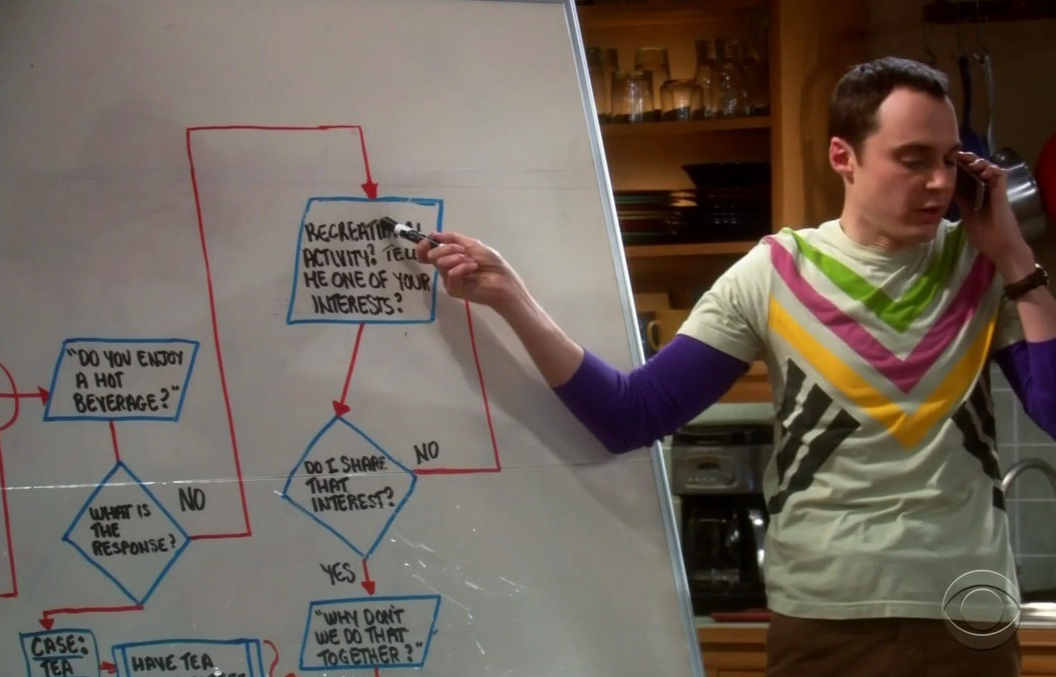
\includegraphics[width=7cm]{fig/Algorithm-sheldon.png}
            }
                 \textit{ I believe I've isolateblblblblblblsblbslbslbsl
            sblbslblsblsblblsblbs
            lbslblbslsb d the algorithm for making friends.}
     
            
            \small{
            \hfill Sheldon Cooper, 
            
            \hfill in \textit{The Big Band Theory}, Season 2, Episode 13
            }


    \end{columns}

\end{frame}


%%%%%%%%%%%%%%%%%%%%%
\subsection{Introduction}
    \begin{frame}
    \frametitle{Pourquoi faire appel � des algorithmes ?}
    Pour automatiser des t�ches
    
    Exemples :
    \begin{itemize}
    \item M�tier � tisser\\
    \item M�thode de calcul � la main d'une division\\
    \item Recette de cuisine\\
    \item ...\\
    \end{itemize}
    \end{frame}
 
 %%%%%%%%%%%%%%%%%
 
    \begin{frame}
    \frametitle{Qu'est-ce qu'un algorithme ?}
    \begin{block}{D�finition}
    Un algorithme est un ensemble 
    ordonn� d'instructions simples
permettant de r�soudre un probl�me.
    \end{block}
    \end{frame}
    
 %%%%%%%%%%%%%%%%%%
 \subsection{Construction d'un algorithme}
%%%%%%%%%%%%%%%%%%%    
\section{La machine de Turing}
%%%%%%%%%%%%%%%%%%%%
 
  
\begin{frame}[fragile]
\frametitle{Un peu d'histoire...}
\begin{codeblock}{Test}
\begin{codeC}
for (int i = 0 ; i < n ; i ++) {
    //a comment
    printf("%d",i);
    }
\end{codeC}
\end{codeblock}

\begin{termblock}{test 2}
\lstset{escapeinside={��}}
\begin{lstlisting}
�\textbf{>>}�./a.out
�\color{darkgray}{\texttt{  Hello World}}�
\end{lstlisting}
\end{termblock}

 \begin{block}{Bloc standard}
blablabla
\end{block}
\end{frame}


\begin{frame}[fragile]
\frametitle{essai}
\begin{columns}
\column{6cm}
\begin{block}

\begin{figure}
\begin{tikzpicture} [
    auto,
    decision/.style = { diamond, draw=blue, thick, fill=blue!20,
                        text width=5em, text badly centered,
                        inner sep=1pt, rounded corners },
    block/.style    = { rectangle, draw=blue, thick, 
                        fill=blue!20, text width=10em, text centered,
                        rounded corners, minimum height=2em },
    line/.style     = { draw, thick, ->, shorten >=2pt },
  ]
   \matrix [column sep=-10mm, row sep=10mm] {
                    & \node [text centered] (x) {$\mathbf{X}$};            & \\
                    & \node (null1) {};                                    & \\
                    & \node [block] (doa) {\textsf{DoAE}($\mathbf{X}$)};   & \\
  	               \node(null3){}; & \node [decision] (uiddes)
                        {\textsf{UID}($\hat{\mathbf{X}}$)};
                                  & \node[text centered](tra){$\mathbf{i}$}; \\
                  & \node [block] (track) {\textsf{DoAT}($\mathbf{x}$)}; & \\
                    & \node [block] (pesos)
                        {\textsf{BF}(DoA$_{\mathrm{T}}$,DoAs)};            & \\
                    & \node [block] (filtrado)
                        {\textsf{SF}($\mathbf{w}$,$\mathbf{x}$)};          & \\
                    & \node [text centered] (xf) {$\hat{x}(t)$ };          & \\
  };
  % connect all nodes defined above
 \begin{scope} [every path/.style=line]
    \path (x)        --    (doa);
    \path (doa)      --    node [near start] {DoAs} (uiddes);
    \path (tra)      --    (uiddes);
    \path (uiddes)   --++  (-3,0) node [near start] {no} |- (null1);
    \path (uiddes)   --    node [near start] {DoA} (track);
    \path (track)    --    node [near start] {DoA$_{\mathrm{T}}$} (pesos);
    \path (pesos)    --    node [near start] {\textbf{w}} (filtrado);
    \path (filtrado) --    (xf);
  
  \end{scope}
\end{tikzpicture}
\end{figure}
\end{block}
\column{3cm}
\begin{block}{bulbul}
\end{block}
\end{columns}
\end{frame}

\end{document}
